\documentclass[12pt,pdf,hyperref={unicode}]{beamer}


%\documentclass[10pt]{beamer}

\usetheme[progressbar=frametitle]{metropolis}

\usepackage{booktabs}
\usepackage[scale=2]{ccicons}

\usepackage{pgfplots}
\usepgfplotslibrary{dateplot}

\usepackage{xspace}
\newcommand{\themename}{\textbf{\textsc{metropolis}}\xspace}


%\usepackage{lmodern}

% подключаем кириллицу 
\usepackage[T2A]{fontenc}
\usepackage[utf8]{inputenc}
\usepackage{listings}
%\usepackage{graphicx}
\usepackage{hyperref}

% отключить клавиши навигации
\setbeamertemplate{navigation symbols}{}

% тема оформления
\usetheme{Pittsburgh}

% цветовая схема
\usecolortheme{default}

\definecolor{light-gray}{gray}{0.90}




\title{Семинар №1}   
\subtitle{ФАКИ \the\year}
\author{Бирюков В. А.} 
\date{\today} 
% \logo{
\includegraphics[height=5mm]{images/logo.pg}\vspace{-7pt}}

\begin{document}

% титульный слайд
\begin{frame}
\titlepage
\end{frame} 

\defverbatim[colored]\makeset{
\begin{lstlisting}[language=C++,basicstyle=\ttfamily,keywordstyle=\color{blue}]
void make_set(int X) {
  parent[X] = X;
}
\end{lstlisting}
}

\lstset{
  language=C,                % choose the language of the code
  basicstyle=\ttfamily,
  columns=fixed,
  fontadjust=true,
  basewidth=0.5em,
  keywordstyle=\color{blue}\bfseries,
  commentstyle=\color{gray},
  stringstyle=\ttfamily\color{yellow!40!red},
  showstringspaces=false,
  %numbers=false,                   % where to put the line-numbers
  numbersep=5pt,
  numberstyle=\tiny\color{gray},
  numberfirstline=true,
  stepnumber=1,                   % the step between two line-numbers.        
  numbersep=5pt,                  % how far the line-numbers are from the code
  backgroundcolor=\color{white!90!gray},  % choose the background color. You must add \usepackage{color}
  showstringspaces=false,         % underline spaces within strings
  captionpos=b,                   % sets the caption-position to bottom
  breaklines=true,                % sets automatic line breaking
  breakatwhitespace=true,         % sets if automatic breaks should only happen at whitespace
}
\lstset{literate=%
   *{0}{{{\color{red!20!violet}0}}}1
    {1}{{{\color{red!20!violet}1}}}1
    {2}{{{\color{red!20!violet}2}}}1
    {3}{{{\color{red!20!violet}3}}}1
    {4}{{{\color{red!20!violet}4}}}1
    {5}{{{\color{red!20!violet}5}}}1
    {6}{{{\color{red!20!violet}6}}}1
    {7}{{{\color{red!20!violet}7}}}1
    {8}{{{\color{red!20!violet}8}}}1
    {9}{{{\color{red!20!violet}9}}}1
}

\begin{frame}
\frametitle{Учебные материалы} 
    \begin{itemize}
    \item CS50 (просто загуглить)
    \item K\&R: Брайан У. Керниган, Деннис М. Ритчи "Язык программирования C"
    \item Томас Кормен, Чарльз Лейзерстон, Рональд Ривест, Клиффорд Штайн "Алгоритмы: построение и анализ"
    \end{itemize}
\end{frame}


\iffalse
\begin{frame}
\frametitle{Linux} 
\begin{columns}
\begin{column}{0.4\textwidth}
   
\includegraphics[width=0.75\linewidth]{tux.png}
\end{column}
\begin{column}{0.6\textwidth}  %%<--- here
    \begin{itemize}
    \item Первая версия ядра Linux -- Линус Торвальдс, 1991 год
    \item Общее название Unix-подобных операционных систем, основанных на ядре Linux
    
    \end{itemize}
\end{column}
\end{columns}
\end{frame}
\fi

\section{Основы командной строки Linux}
\begin{frame}
\frametitle{Основы командной строки} 
\framesubtitle{Основные команды}
\begin{description}
  \item[pwd (сокращение от personal working directory)] \hfill \\
  \item[ls (сокращение от list)] \hfill \\
  Опции: -l, -a
  \item[cd (change directory)] \hfill \\
  Применение: cd <имя директории> \\
  Особые директории: . ..  $\sim$
  \item[man (manual)] \hfill \\
  Применение: man <имя команды>\\
  Например: man ls
\end{description}
\end{frame}

\begin{frame}
\frametitle{Основы командной строки} 
\framesubtitle{Основные команды}
\begin{description}
  \item[cp (copy)] \hfill \\
  Применение: cp <источник> <назначение>
  \item[mv (move)] \hfill \\
  Применение: mv <источник> <назначение>\\
  Можно переименовывать файлы
  \item[rm (remove)] \hfill \\
  Применение: rm <имя файла> \\
  Чтобы удалить директорию: опция -r\\
  Будьте осторожны!
\end{description}
\end{frame}

\begin{frame}
\frametitle{Основы командной строки} 
\framesubtitle{Основные команды}
\begin{description}
  \item[mkdir (make directory)] \hfill \\
  Применение: mkdir <название директории>
  \item[nano - текстовый редактор] \hfill \\
  nano ./<имя\_файла>\\
  Ctrl + X - закрыть редактор\\
  Ctrl + O - сохранение файла
  \item[vim - продвинутый текстовый редактор] \hfill \\
  vim ./<имя\_файла>\\
  i - перейти в режим редактирования\\
  ESC - выйти из режима редактирования\\
  :wq и :q! - выйти с сохранением и без сохранения соответственно
\end{description}
\end{frame}


\section{Helloworld. Компилятор gcc.}


\begin{frame}[fragile]
\frametitle{Пример простейшей программы на языке C}
Программа, которая ничего не делает \\
\begin{lstlisting}[language=C++,basicstyle=\ttfamily,keywordstyle=\color{blue}]
int main()
{
}
\end{lstlisting}
Функция main -- начальная точка выполнения для всех С и C++ программ
\end{frame}

\begin{frame}[fragile]
\frametitle{Helloworld} 
\framesubtitle{Программа, которая печатает Helloworld на экран} 
\begin{center}
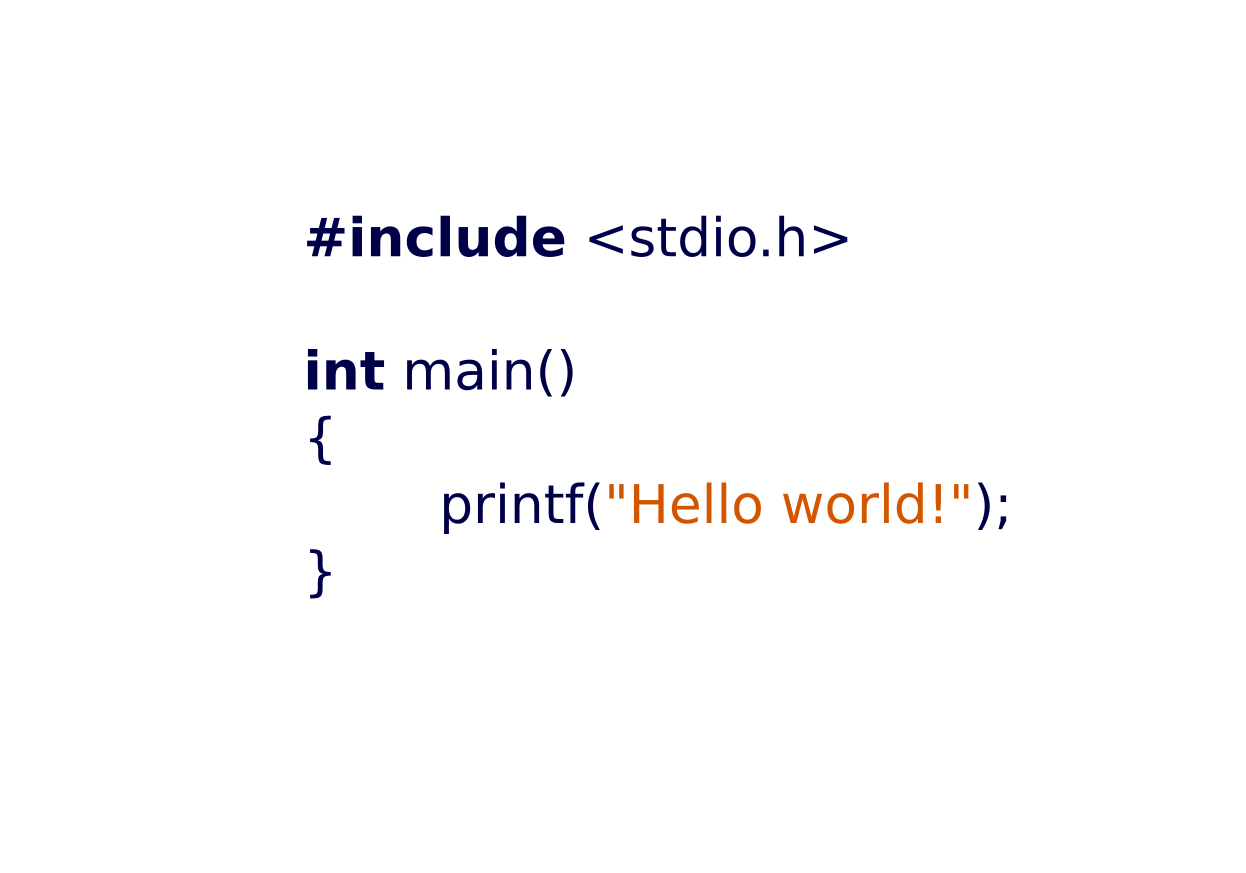
\includegraphics[width=0.99\linewidth]{images/hw1.png}
\end{center}
\end{frame}

\begin{frame}[fragile]
\frametitle{Helloworld} 
\framesubtitle{Программа, которая печатает Helloworld на экран} 
\begin{center}
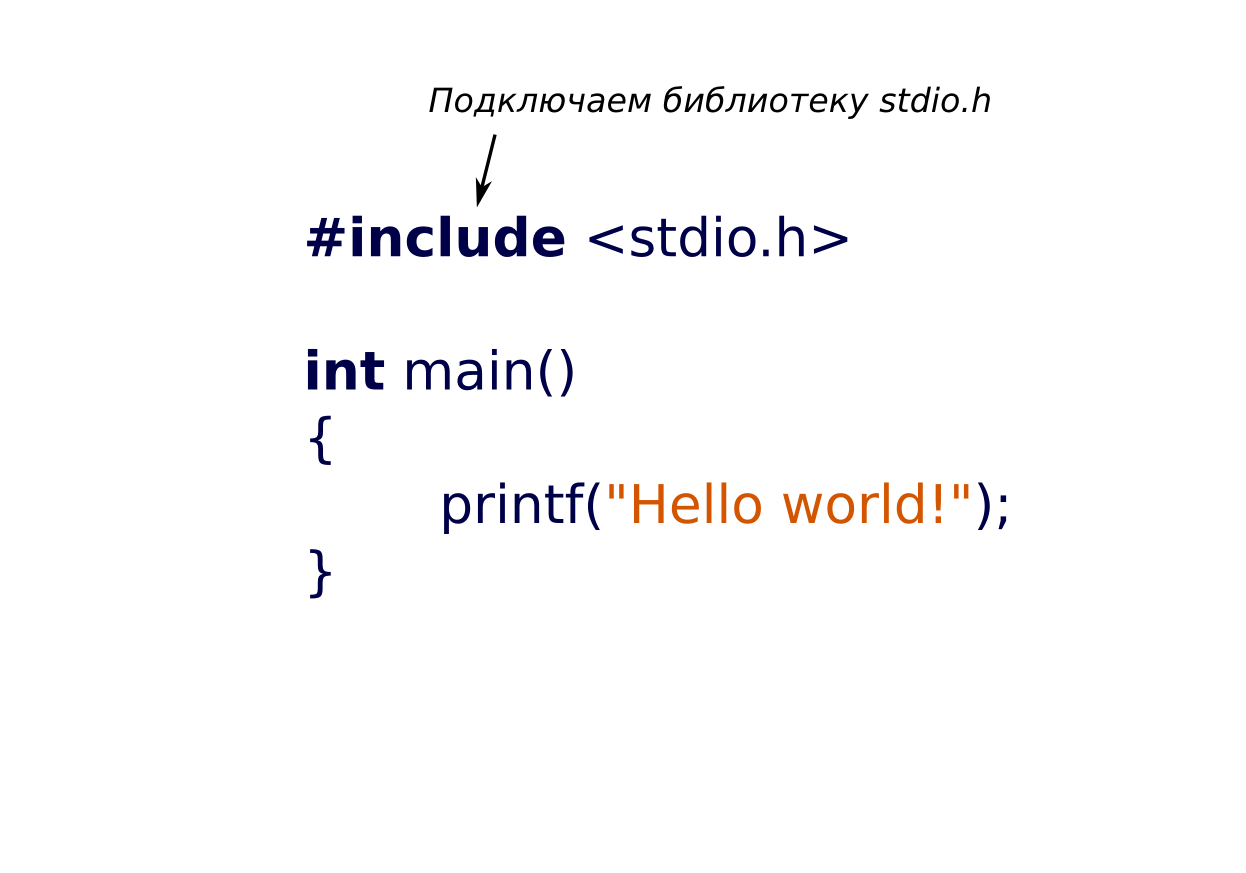
\includegraphics[width=0.99\linewidth]{images/hw2.png}
\end{center}
\end{frame}

\begin{frame}[fragile]
\frametitle{Helloworld} 
\framesubtitle{Программа, которая печатает Helloworld на экран} 
\begin{center}
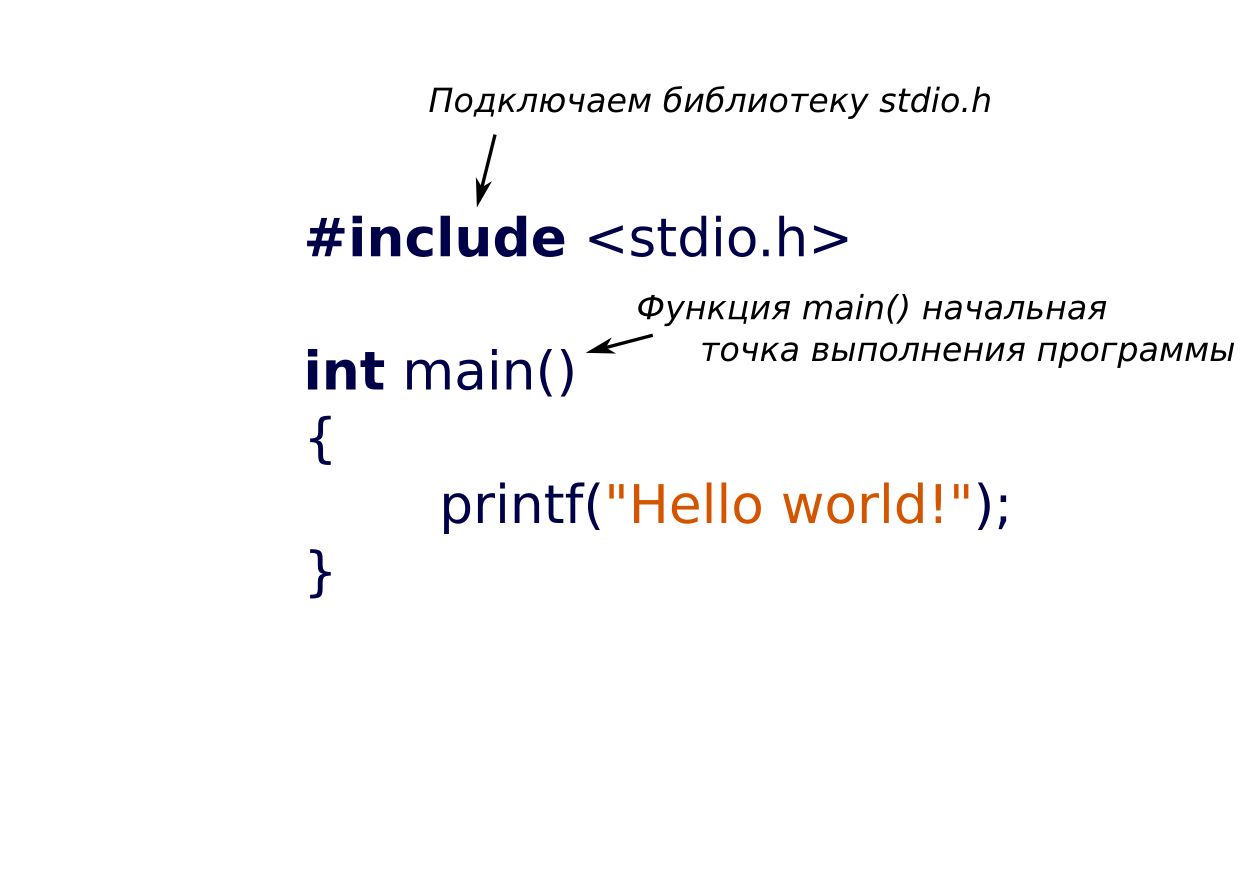
\includegraphics[width=0.99\linewidth]{images/hw3.png}
\end{center}
\end{frame}


\begin{frame}[fragile]
\frametitle{Helloworld} 
\framesubtitle{Программа, которая печатает Helloworld на экран} 
\begin{center}
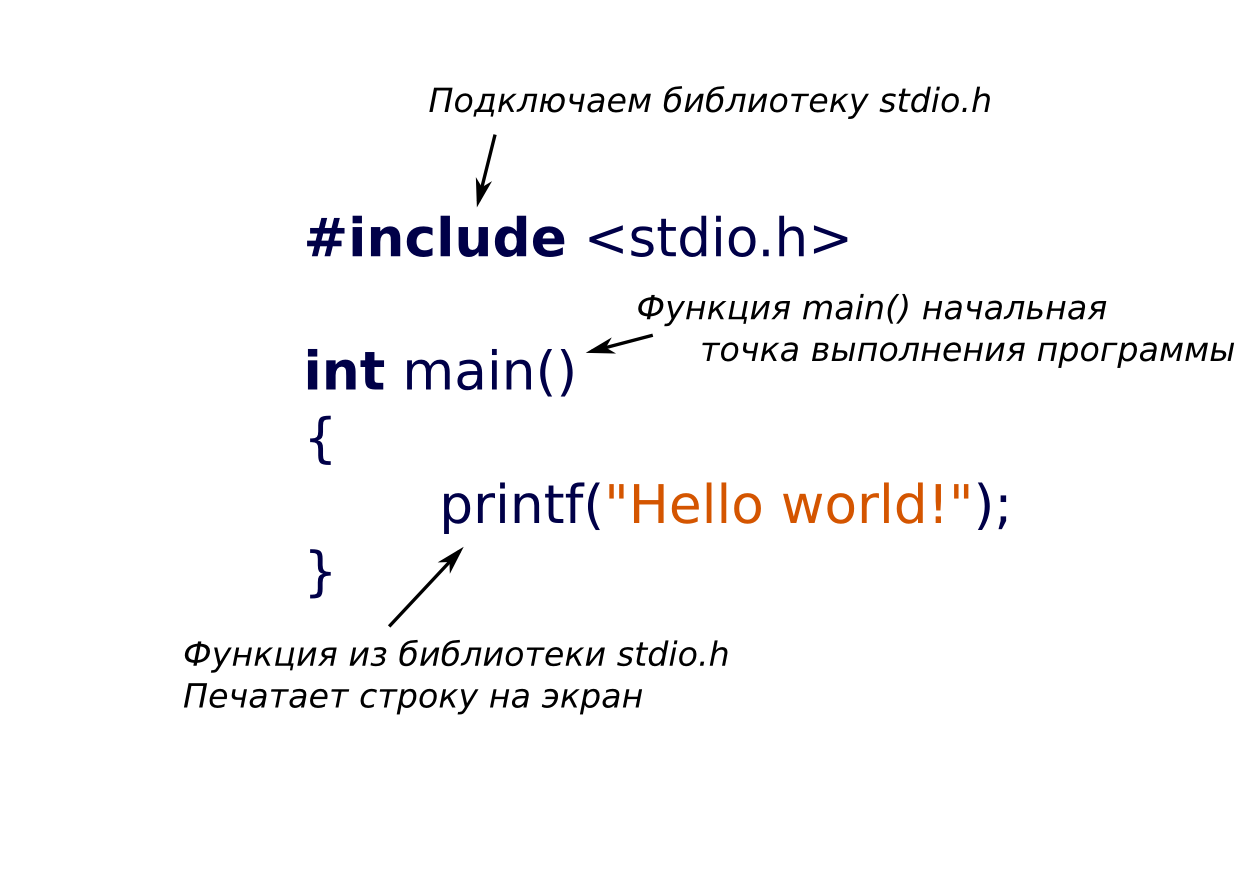
\includegraphics[width=0.99\linewidth]{images/hw4.png}
\end{center}
\end{frame}

\begin{frame}[fragile]
\frametitle{Helloworld} 
\framesubtitle{Программа, которая печатает Helloworld на экран} 
\begin{center}
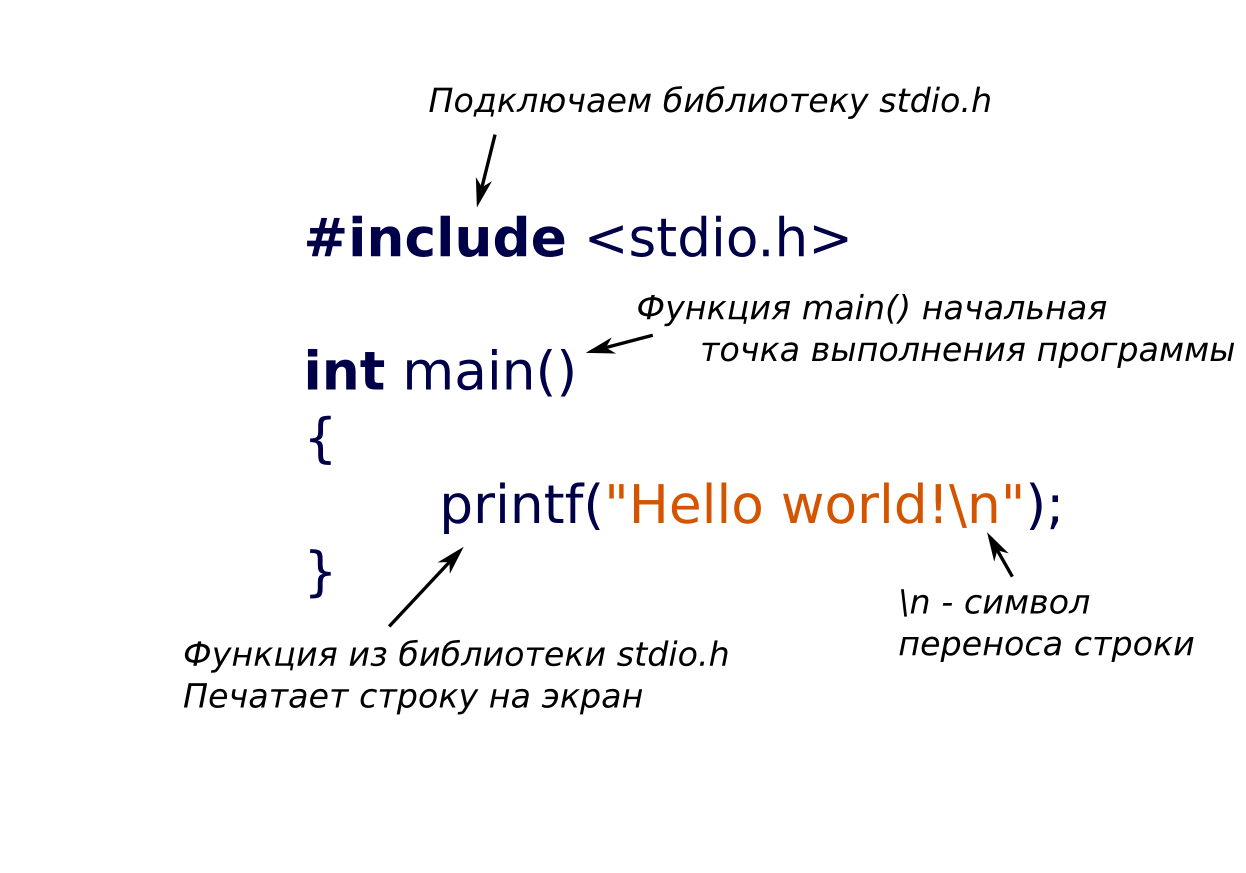
\includegraphics[width=0.99\linewidth]{images/hw5.png}
\end{center}
\end{frame}



\begin{frame}
\frametitle{Компилятор gcc}
\begin{description}
  \item[gcc (GNU Compiler Collection)] \hfill \\
  gcc <имя файла для компиляции>\\
  -o -- задать имя файла \\
  Имя файла по умолчанию: a.out \\
  Примеры: \\
  \quad  \textbf{gcc -o hello hello.c} \\
  Скомпилирует файл hello.c и создаст исполняемый файл hello, который можно будет запустить исполнив ./hello
\end{description}
\end{frame}


\section{Основы языка C. Базовые типы и операторы.}

\begin{frame}
\frametitle{Особенности языка C:} 
\begin{center}
\begin{itemize}
\item Простой синтаксис
\item Простой доступ к памяти, указатели
\item Низкоуровневый
\item Очень быстрый
\item Небезопасный
\item Сложно писать большие программы
\end{itemize}
\end{center}
\end{frame}


\begin{frame}
\frametitle{Переменные} 
\begin{center}
\begin{itemize}
\item Именованная область памяти, адрес которой можно использовать для осуществления доступа к данным
\item Название переменной может содержать латинские буквы, цифры и \_, но не может начинаться с цифры
\end{itemize}
\end{center}
\end{frame}


\begin{frame}[fragile]
\frametitle{Память и переменные} 
\framesubtitle{Объявление переменной типа int(целое число)} 
\begin{center}
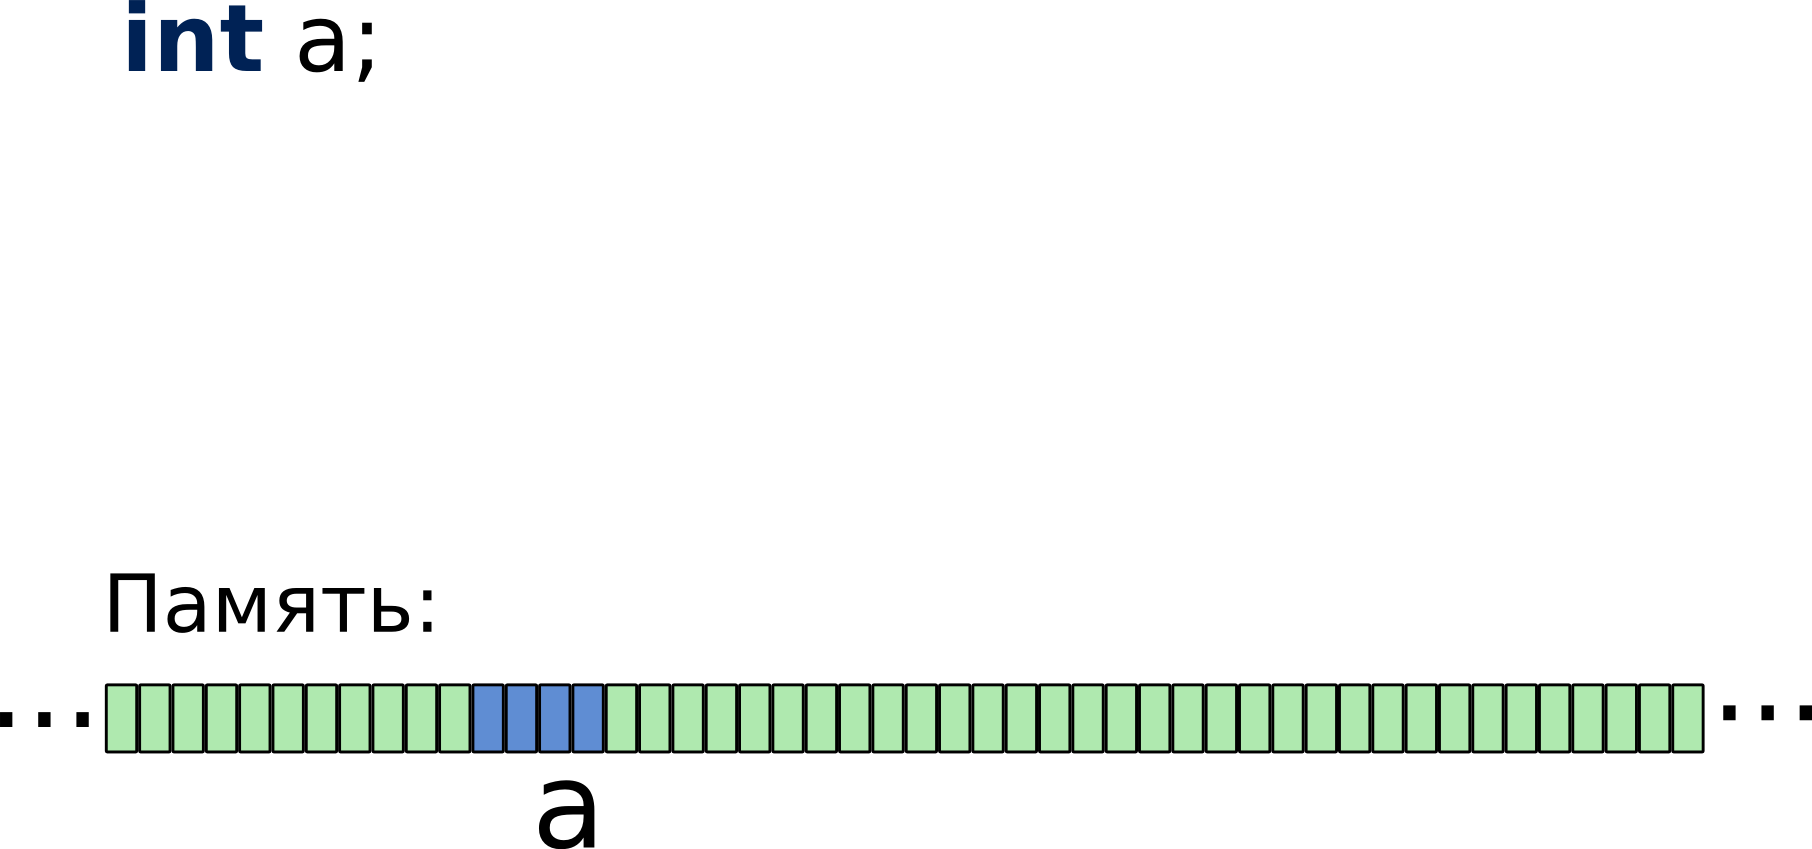
\includegraphics[width=0.99\linewidth]{images/memory1.png}
\end{center}
\end{frame}

\begin{frame}[fragile]
\frametitle{Память и переменные} 
\framesubtitle{Объявление переменной типа int(целое число)} 
\begin{center}
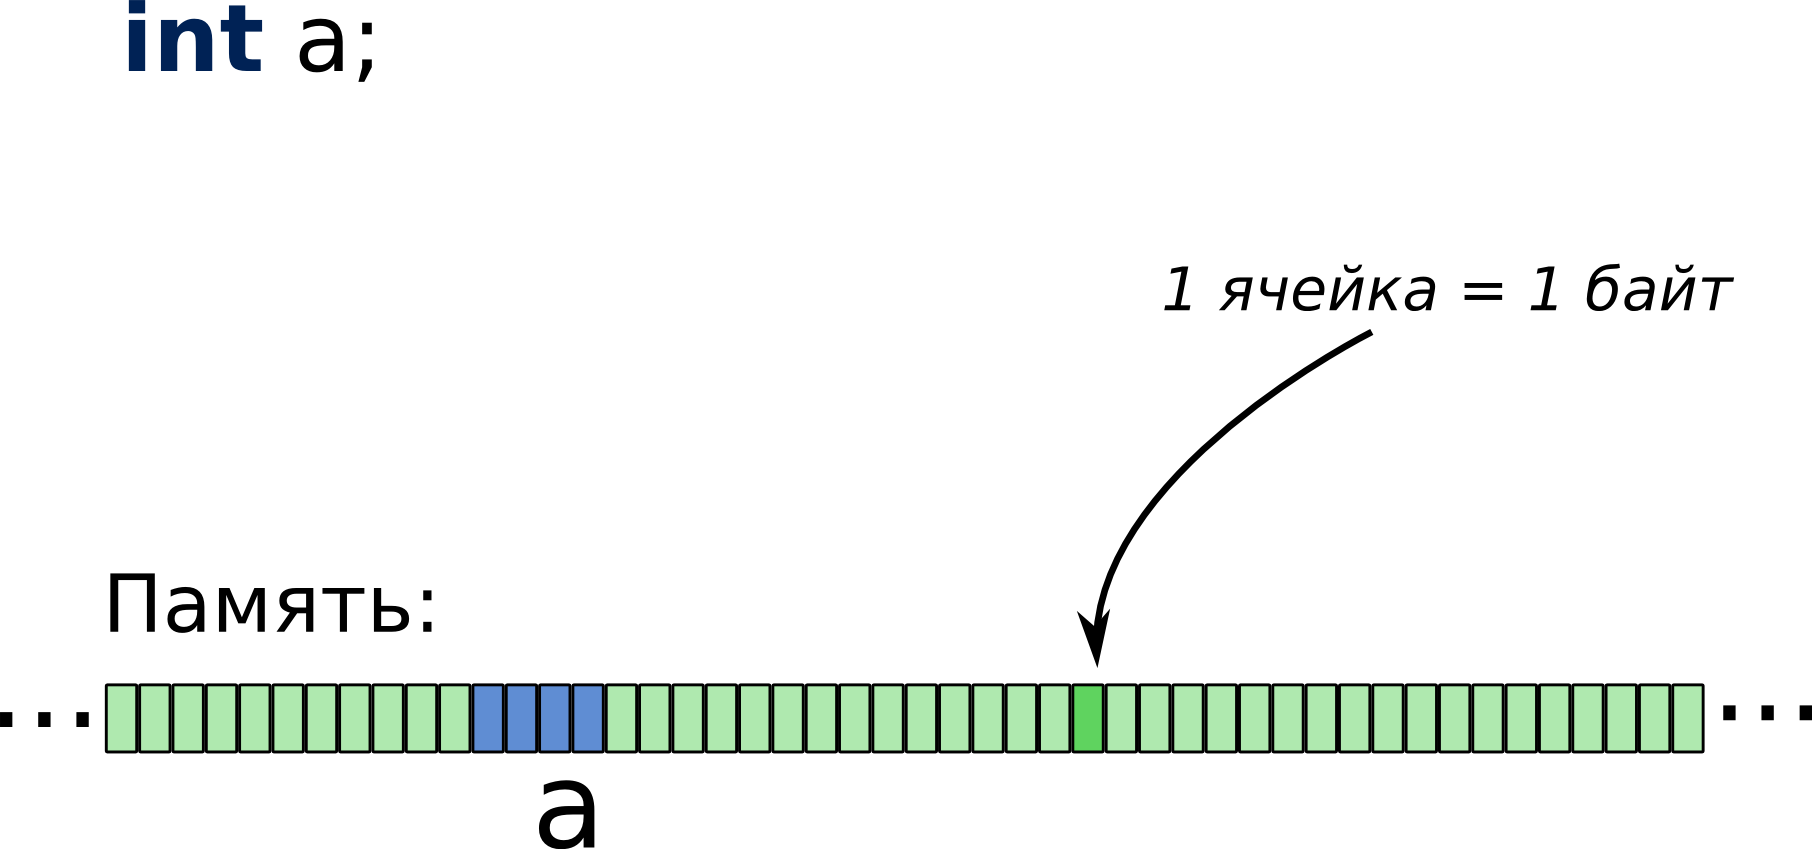
\includegraphics[width=0.99\linewidth]{images/memory2.png}
\end{center}
\end{frame}

\begin{frame}[fragile]
\frametitle{Память и переменные} 
\framesubtitle{Объявление переменной типа int(целое число)} 
\begin{center}
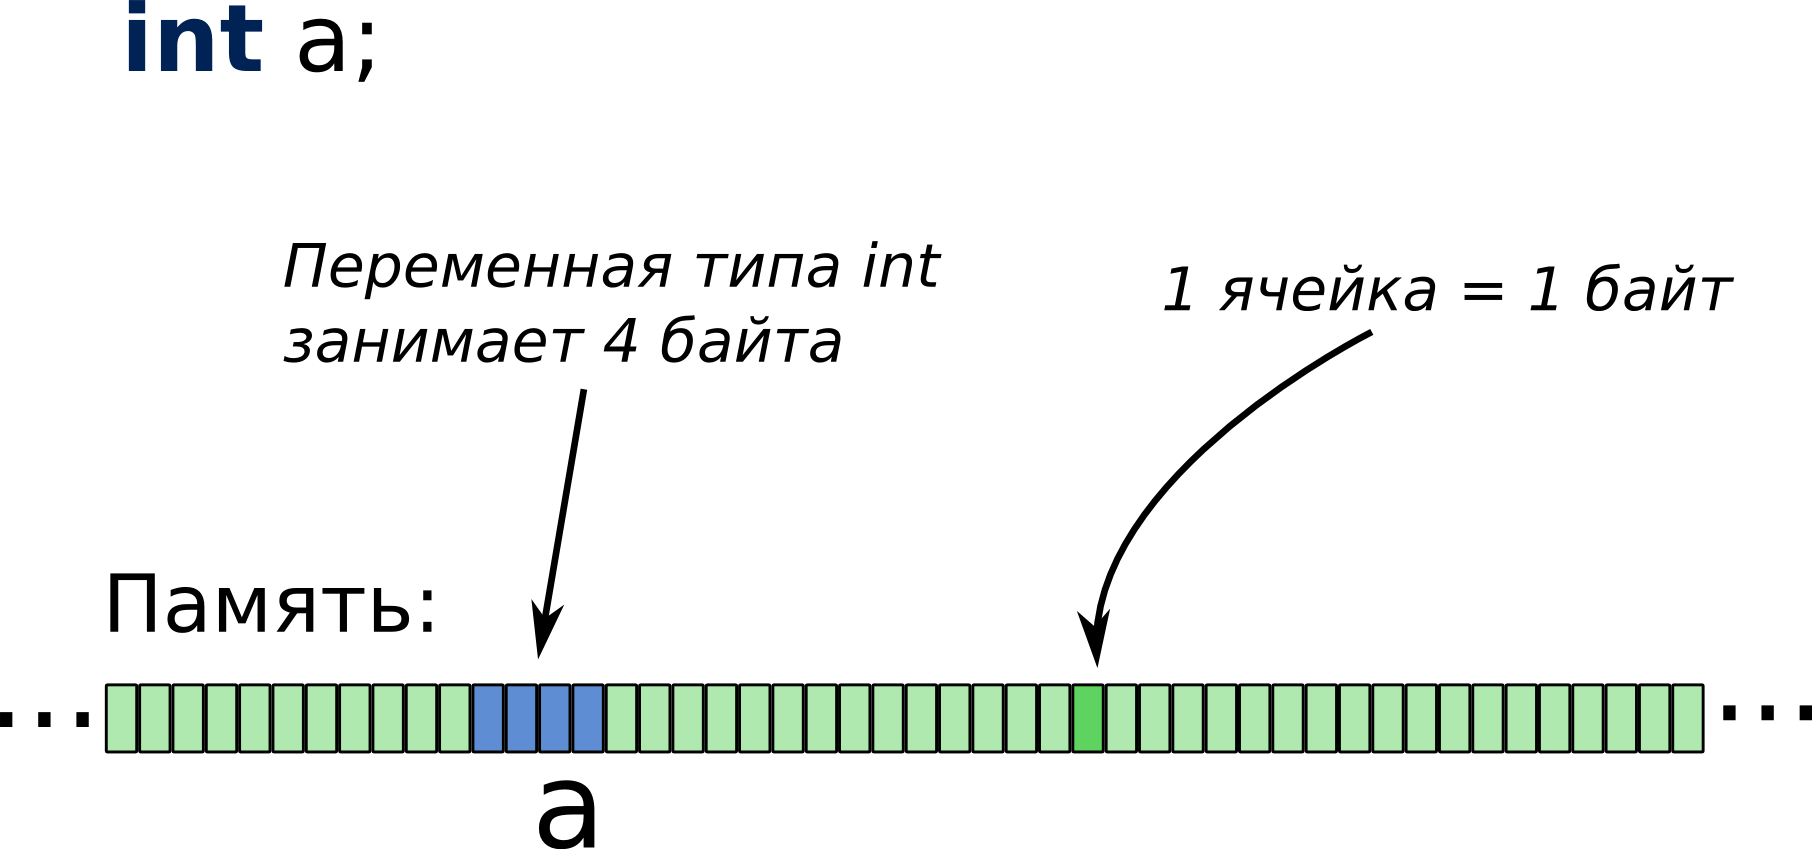
\includegraphics[width=0.99\linewidth]{images/memory3.png}
\end{center}
\end{frame}

\begin{frame}[fragile]
\frametitle{Память и переменные} 
\framesubtitle{Объявление переменной типа int и float(вещественное число)} 
\begin{center}
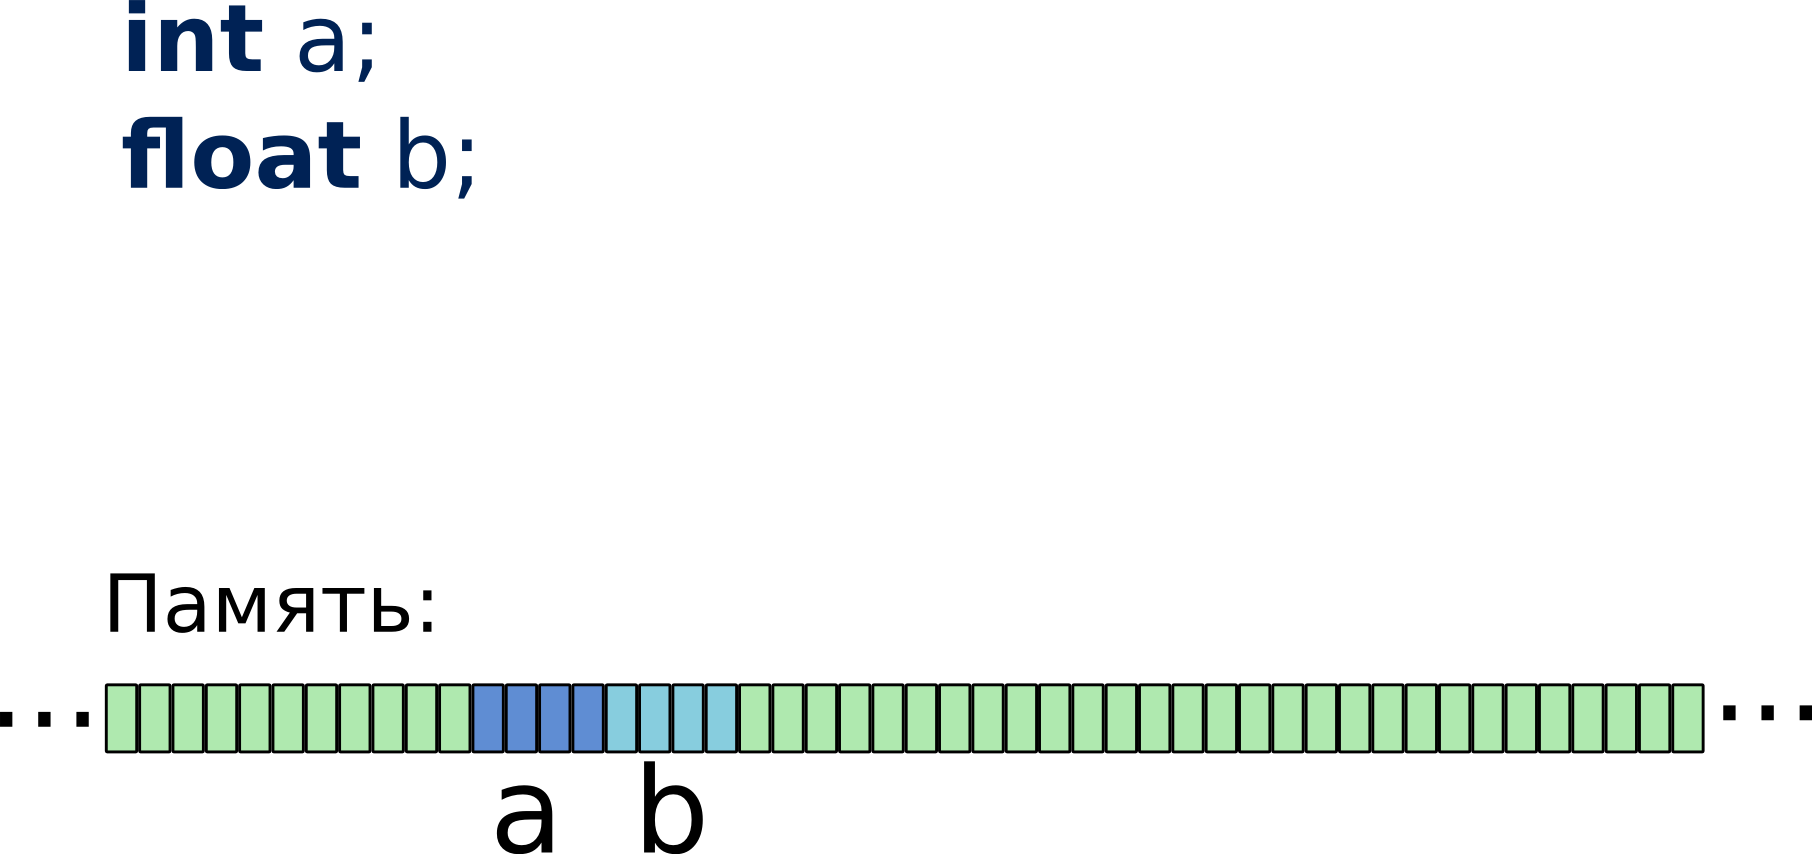
\includegraphics[width=0.99\linewidth]{images/memory4.png}
\end{center}
\end{frame}

\begin{frame}[fragile]
\frametitle{Память и переменные} 
\framesubtitle{Объявление  int, float и char(целое число размером 1 байт)} 
\begin{center}
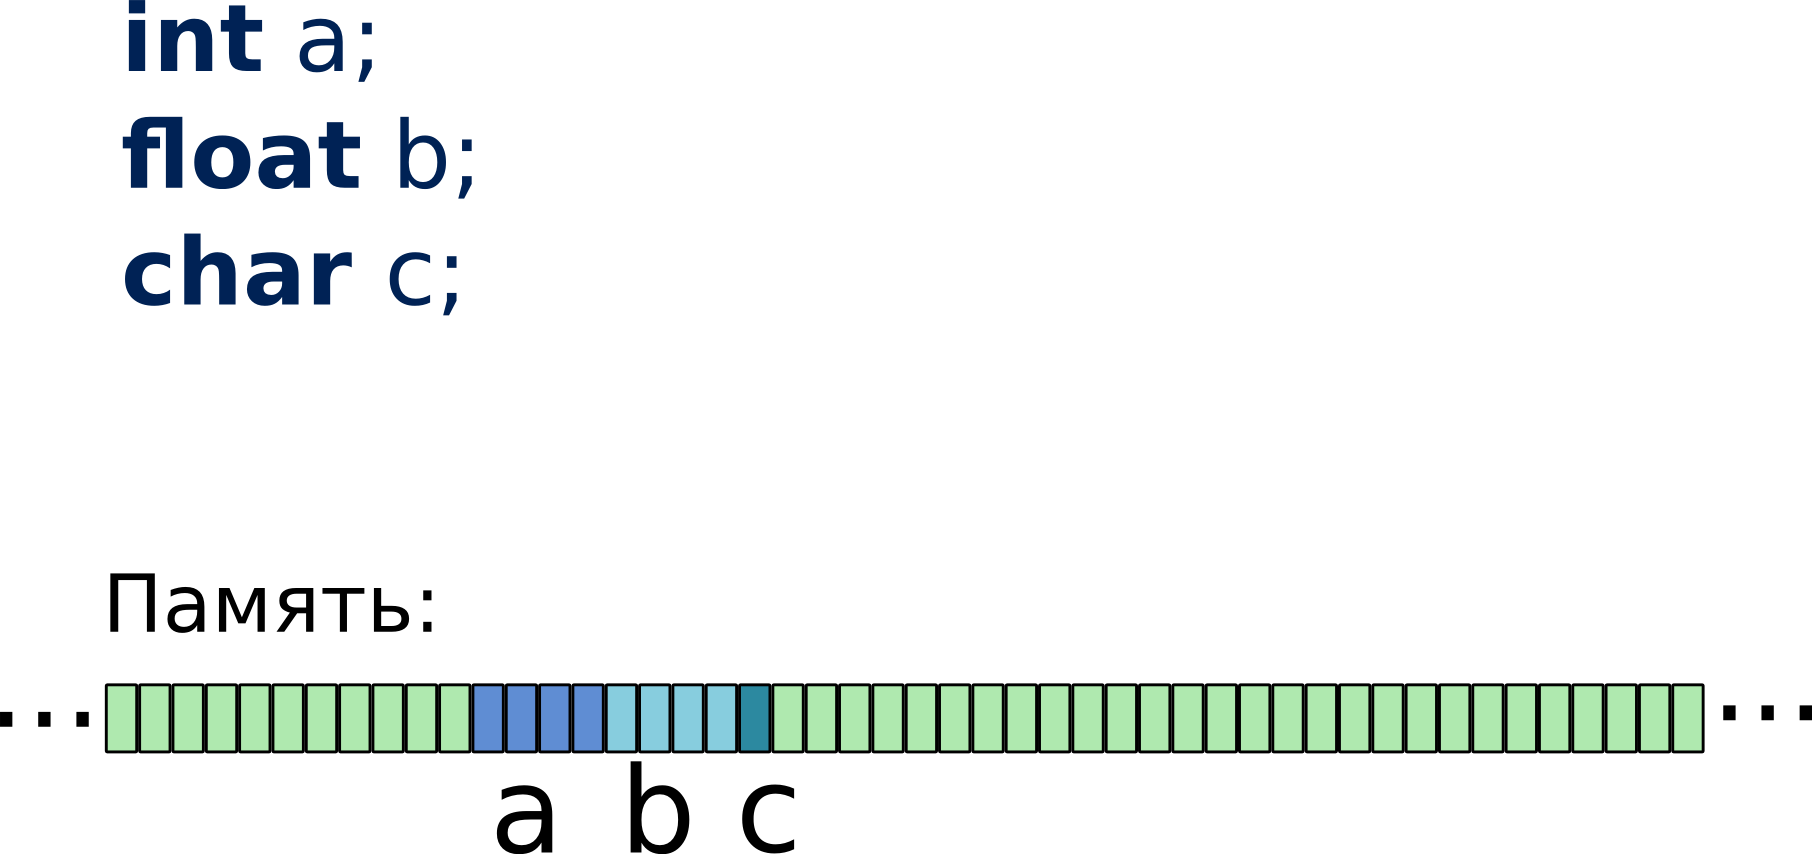
\includegraphics[width=0.99\linewidth]{images/memory5.png}
\end{center}
\end{frame}

\begin{frame}[fragile]
\frametitle{Память и переменные} 
\framesubtitle{Инициализация переменной. (big-endian)} 
\begin{center}
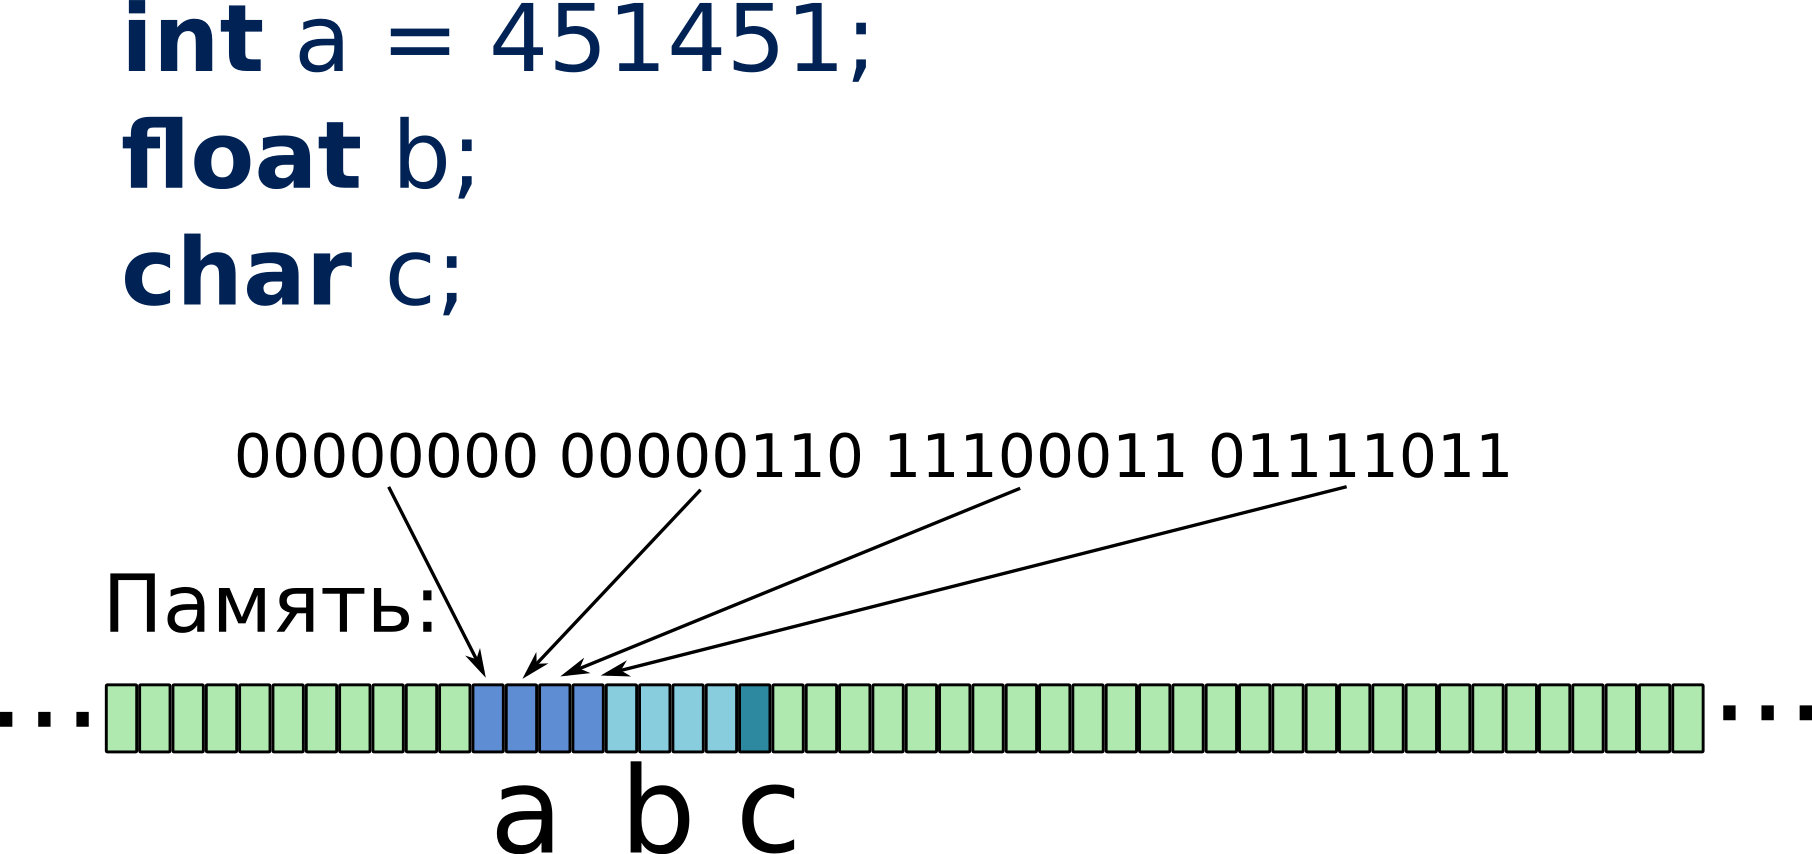
\includegraphics[width=0.99\linewidth]{images/memory6.png}
\end{center}
\end{frame}

\begin{frame}[fragile]
\frametitle{Память и переменные} 
\framesubtitle{Адреса переменных} 
\begin{center}
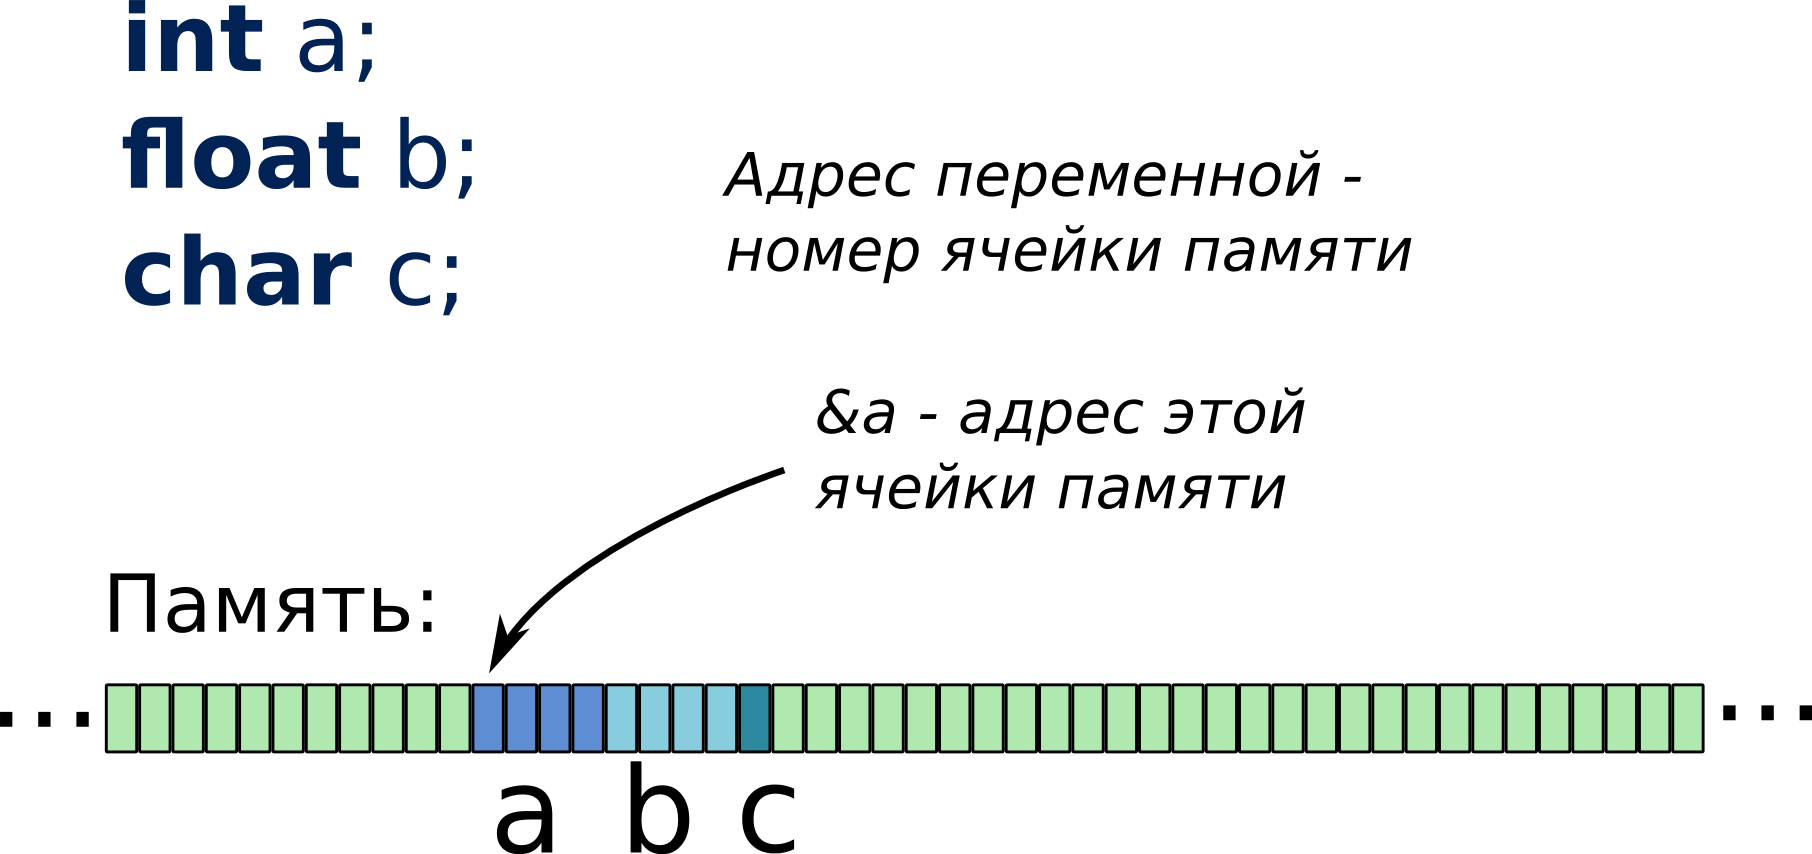
\includegraphics[width=0.99\linewidth]{images/memory7.png}
\end{center}
\end{frame}

\begin{frame}[fragile]
\frametitle{Память и переменные} 
\framesubtitle{Адреса переменных} 
\begin{center}
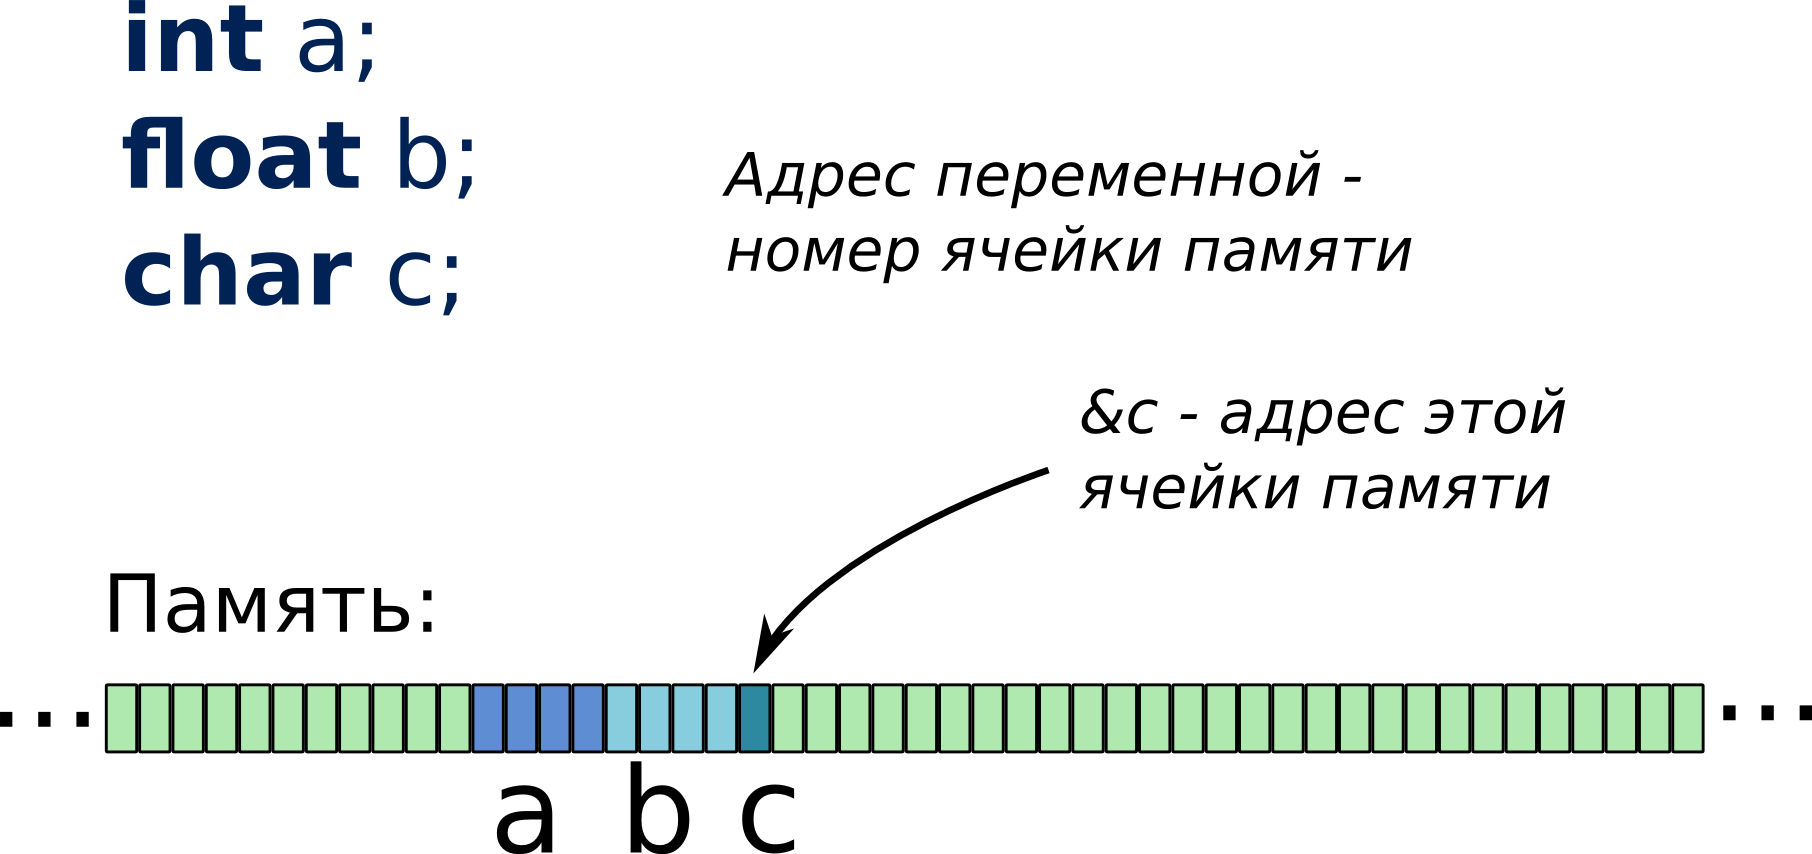
\includegraphics[width=0.99\linewidth]{images/memory8.png}
\end{center}
\end{frame}

\iffalse
\begin{frame}
\frametitle{Объявление переменных} 
\begin{center}
\begin{itemize}
\item Переменную нужно объявить перед использованием
\item Примеры объявления:\\
\textcolor{blue}{\textbf{int}} n;\\
\textcolor{blue}{\textbf{float}} p;
\item int -- целочисленный тип \\
\item float -- тип чисел с плавающей точкой
\end{itemize}
\end{center}
\end{frame}

\begin{frame}
\frametitle{Инициализация переменных} 
\begin{center}
\begin{itemize}
\item Переменные инициализируются с помощью оператора присваивания =
\item Примеры:\\
\textcolor{blue}{\textbf{float}} p = 5.4; \\
\textcolor{blue}{\textbf{int}} a = 15, b = 5, c = 9;
\end{itemize}
\end{center}
\end{frame}
\fi

\begin{frame}
\frametitle{Базовые типы}
\frametitle{Целочисленные типы} 
\begin{center}
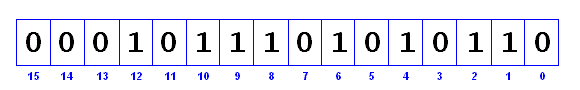
\includegraphics[scale=0.5]{images/bit_positions.png}
\end{center}
Число бит на тип зависит от системы. Для 64-х битных:
\begin{center}
\begin{tabular}{ l c l }
  Название типа & Число бит & Макс. значения \\
  char & 8 & -128..127 или 0..255 \\
  short & 16 & -32768..32767 \\
  int & 32 & $-2 \cdot 10^9$ ..$+2 \cdot 10^9$ \\
  long int & 64& $-2^{63}$ ..$+2^{63}-1$ \\
  long long int & 64 & $-2^{63}$ ..$+2^{63}-1$ \\
\end{tabular}
\end{center}
\end{frame}

\begin{frame}
\frametitle{Базовые типы}
\frametitle{Беззнаковые целочисленные типы} 
Число бит на тип зависит от компилятора. Обычные значения такие:
\begin{center}
\begin{tabular}{ l c l }
  Название типа & Число бит & Макс. значения \\
  unsigned char & 8 & 0..255 \\
  unsigned short & 16 & 0..65535 \\
  unsigned int & 32 & $0$ ..$+4 \cdot 10^9$ \\
  unsigned long int & 64& $0$ ..$+2^{64}-1$ \\
  unsigned long long int & 64 & $0$ ..$+2^{64}-1$ \\
\end{tabular}
\end{center}
sizeof() -- размер файла в байтах
\end{frame}


\begin{frame}
\frametitle{Базовые типы}
\frametitle{Типы чисел с плавающей точкой} 
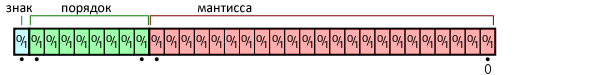
\includegraphics[scale=0.6]{images/floats.png}
\begin{center}
\begin{tabular}{ l c l }
  Название типа & Число бит & Макс. значения \\
  float & 32 & $10^{-38}$..$10^{+38}$ \\
  double & 64 & $10^{-308}$..$10^{+308}$ \\
\end{tabular}
\end{center}
Обычно используется double, так как float может быть недостаточно точен
\end{frame}

\begin{frame}
\frametitle{Базовые операторы}
\frametitle{Оператор присваивания =} 
Присваивает переменной значение:\\
Пример:\\
\quad \textcolor{blue}{int} a, b;\\
\quad \textcolor{blue}{float} c, d;\\
\quad a = 1;\\
\quad b = a + 1;\\
\quad c = 5.6;\\
\quad d = 19;\\
\quad a = 4.6;\\

\end{frame}


\begin{frame}
\frametitle{Базовые операторы}
\frametitle{Математические операторы: + - / * \%} 
Примеры:\\
\quad a = 1 + 1; \\
\quad b = 5.0 / 2.0;\\
\quad c = 5 / 2;\\
\quad d = 5 \% 2;\\
\end{frame}

\begin{frame}
\frametitle{Базовые операторы}
\frametitle{Унарные операторы: + - ++ - -}
Оператор инкремента ++ -- увеличивает значение переменной на 1 и присваевает переменной  \\
Примеры:\\
\quad a = +5; \\
\quad b = -a;\\
\quad c = ++a;\\
\quad d = c++;\\
\end{frame}







\iffalse

\begin{frame}
\frametitle{Базовые операторы}
\frametitle{Операторы отношения}
Возвращают тип bool
\begin{center}
\begin{tabular}{ l l}
  == & равно \\
  != & не равно \\
  > & больше \\
  >= & больше или равно \\
  < & меньше \\
  <= & меньше или равно \\
\end{tabular}
\end{center}

Не путайте оператор присваивания = и оператор сравнения == !! 
\end{frame}


\begin{frame}
\frametitle{Базовые операторы}
\frametitle{Логические операторы}
Возвращают тип bool
\begin{center}
\begin{tabular}{ l l}
  ! & не \\
  || & или \\
  \&\& & и \\
\end{tabular}
\end{center}
\end{frame}

\begin{frame}
\frametitle{Базовые операторы}
\frametitle{Побитовые операторы}
\begin{center}
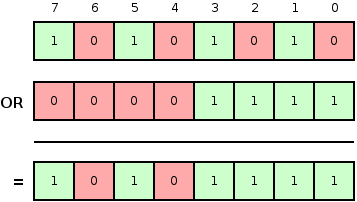
\includegraphics[scale=0.5]{bitwise_or.png}
\end{center}
\begin{center}
\begin{tabular}{ l l}
  $\sim$ & побитовое не \\
  | & побитовое или \\
  \& & побитовое и \\
  \^{} & побитовое исключающее или \\
\end{tabular}
\end{center}
\end{frame}

\begin{frame}
\frametitle{Базовые операторы}
\frametitle{Другие операторы присваивания}
\begin{center}
\begin{tabular}{ l l}
  += & a += b тоже что и a = a + b  \\
  -= & a -= b тоже что и a = a - b  \\
  *= & a *= b тоже что и a = a * b  \\
  |= & a |= b тоже что и a = a | b  \\
  и другие
\end{tabular}
\end{center}
\end{frame}

\begin{frame}
\frametitle{Базовые операторы}
\frametitle{Приоритет операторов}
\begin{center}
\begin{enumerate}
\item (), []
\item ++, --, +, -(унарные), sizeof
\item *, /, \%
\item +, -
\item >,<,<=,>=
\item ==, !=
\item \&, |, \&\&, ||
\item =, +=, и т.д.
\end{enumerate}
\end{center}
Приоритет операторов C подробнее:\\
\href{http://ru.cppreference.com/w/c/language/operator_precedence}
{\textcolor{red}{ru.cppreference.com/w/c/language/operator\_precedence}}
\end{frame}

\fi

\section{Функции printf() и scanf().}

\begin{frame}
\frametitle{Функции printf и scanf.}
printf(строка форматирования, пер1, пер2, ...) \\
scanf(строка форматирования, \&пер1, \&пер2, ...)
\begin{center}
\begin{tabular}{ l l l }
  Обозначение & Типы & Пример \\
  i & Целочисленные типы & 392 \\
  f & Типы с плавающей точкой & 392.5 \\
\end{tabular}
\end{center}
\end{frame}



\iffalse

\begin{frame}
\frametitle{Задание 1} 
\framesubtitle{Конвертер температуры из Фаренгейт в Цельсии} 
\begin{center}
\begin{itemize}
\item Создать переменную типа float \\
\item Считать её значение из стандартного ввода с помощью scanf\\
\item Создать новую переменную типа float и записать преобразованное выражение \\
\item $T_C = \frac{5}{9}(T_F-32)$\\
\item Вывести значение в стандартный вывод с помощью printf\\
\item Скомпилировать программу с помощью gcc и запустить
\end{itemize}
\end{center}
\end{frame}


\begin{frame}
\frametitle{Задание} 
Задачи от hello до sum\_3 включительно.
\end{frame}

\begin{frame}
\frametitle{Задание 2} 
\framesubtitle{Знаки после запятой} 
\begin{center}
\begin{itemize}
\item Пользователь вводит вещественное число $x$ и целое число $n$ \\
\item Нужно вывести $x^5$ c $n$ знаками после запятой\\
\end{itemize}
\end{center}
\begin{center}
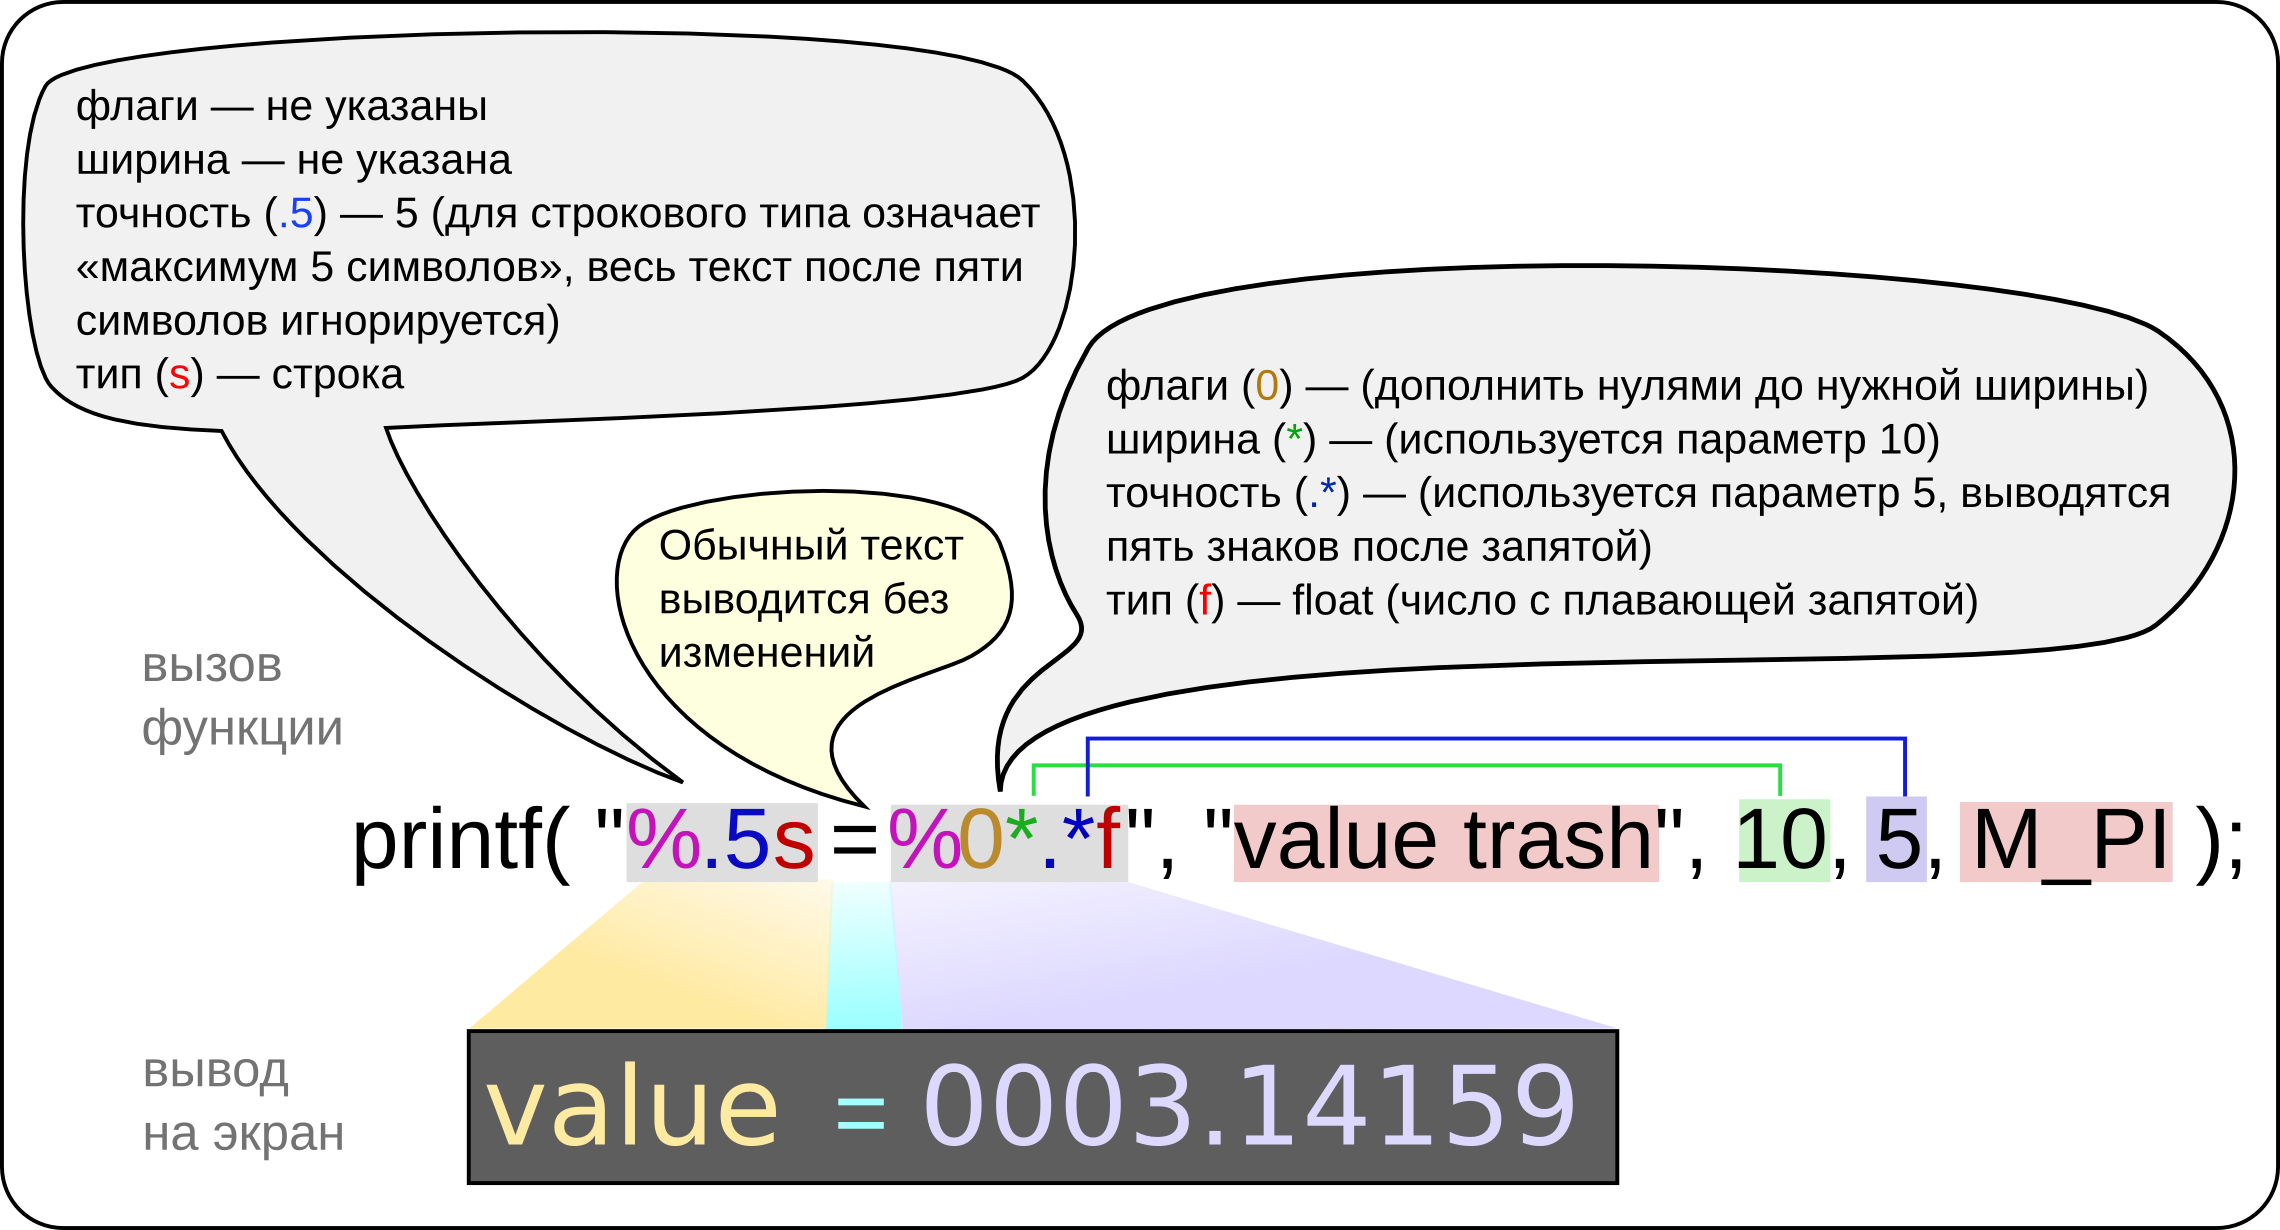
\includegraphics[scale=0.5]{Printf_illustration.png}
\end{center}
\end{frame}

\begin{frame}
\frametitle{Задание 3} 
\framesubtitle{Площадь треугольника} 
\begin{center}
\begin{itemize}
\item Пользователь вводит три пары вещественных чисел -- координаты точек треугольника\\
\item Нужно вывести площадь этого треугольника\\
\item Площадь треугольника можно найти так: $S = \frac{1}{2}|[\vec{r_1} \vec{r_2}]|$\\
\item Где $\vec{r_1}$ и $\vec{r_2}$ -- вектора соответствующие сторонам треугольника.
\item Могут понадобиться функции abs() из stdlib.h или sin() и sqrt() из math.h
\end{itemize}
\end{center}
\end{frame}

\begin{frame}
\frametitle{Задание 4} 
\framesubtitle{Индекс символа} 
\begin{center}
\begin{itemize}
\item Пользователь вводит символ\\
\item Нужно напечатать номер этого символа в кодировке ASCII\\
\item Также нужно напечатать символы и индексы соседних символов в кодировке ASCII \\
\end{itemize}
\end{center}
\end{frame}

\fi


\end{document}
